\documentclass[12pt]{book}
\usepackage[width=4.375in, height=7.0in, top=1.0in, papersize={5.5in,8.5in}]{geometry}
\usepackage[pdftex]{graphicx}
\usepackage{amsmath}
\usepackage{amssymb}
\usepackage{tipa}
%\usepackage{txfonts}
\usepackage{textcomp}
%\usepackage{array}
%\usepackage{xy}
\usepackage{fancyhdr}
\usepackage{tikz}
\usepackage{cancel}

\pagestyle{fancy}
\renewcommand{\chaptermark}[1]{\markboth{#1}{}}
\renewcommand{\sectionmark}[1]{\markright{\thesection\ #1}}
\fancyhf{}
\fancyhead[LE,RO]{\bfseries\thepage}
\fancyhead[LO]{\bfseries\rightmark}
\fancyhead[RE]{\bfseries\leftmark}
\renewcommand{\headrulewidth}{0.5pt}
\renewcommand{\footrulewidth}{0pt}
\addtolength{\headheight}{0.5pt}
\setlength{\footskip}{0in}
\renewcommand{\footruleskip}{0pt}
\fancypagestyle{plain}{%
\fancyhead{}
\renewcommand{\headrulewidth}{0pt}
}
%
%\parindent 0in
\parskip 0.05in

\usepackage{hyperref}
\hypersetup{
	colorlinks=true,
	linkcolor=blue,
	filecolor=magenta
	urlcolor=cyan
	urlstyle{same}
	}
%\href{www.aaa.com}{This Link}

\usepackage{amsthm}
%\newenvironment{theorem}[2][Theorem]{\begin{trivlist}
%\item[\hskip \labelsep {\bfseries #1}\hskip \labelsep {\bfseries #2.}]}{\end{trivlist}}
%\newenvironment{lemma}[2][Lemma]{\begin{trivlist}
%\item[\hskip \labelsep {\bfseries #1}\hskip \labelsep {\bfseries #2.}]}{\end{trivlist}}
%\newenvironment{exercise}[2][Exercise]{\begin{trivlist}
%\item[\hskip \labelsep {\bfseries #1}\hskip \labelsep {\bfseries #2.}]}{\end{trivlist}}
%\newenvironment{example}[2][Example]{\begin{trivlist}
%\item[\hskip \labelsep {\bfseries #1}\hskip \labelsep {\bfseries #2.}]}{\end{trivlist}}
%\newenvironment{Recall}[2][Recall]{\begin{trivlist}
%\item[\hskip \labelsep {\bfseries #1}\hskip \labelsep {\bfseries #2.}]}{\end{trivlist}}
%\newenvironment{remark}[2][Remark]{\begin{trivlist}
%\item[\hskip \labelsep {\bfseries #1}\hskip \labelsep {\bfseries #2.}]}{\end{trivlist}}
%\newenvironment{proposition}[2][Proposition]{\begin{trivlist}
%\item[\hskip \labelsep {\bfseries #1}\hskip \labelsep {\bfseries #2.}]}{\end{trivlist}}
%\newenvironment{corollary}[2][Corollary]{\begin{trivlist}
%\item[\hskip \labelsep {\bfseries #1}\hskip \labelsep {\bfseries #2.}]}{\end{trivlist}}
%\newenvironment{definition}[2][Definition]{\begin{trivlist}
%\item[\hskip \labelsep {\bfseries #1}\hskip \labelsep {\bfseries #2.}]}{\end{trivlist}}

%\theoremstyle{definition}
%\newtheorem{definition}{Definition}
%\newtheorem*{definition*}{Definition}
%\newtheorem{remark}{Remark}
%\newtheorem*{remark*}{Remark}
%\newtheorem{example}{Example}
%\newtheorem*{example*}{Example}
%\newtheorem{exercise}{Exercise}
%\newtheorem*{exercise*}{Exercise}
%
%\theoremstyle{plain}
%\newtheorem{theorem}{Theorem}
%\newtheorem*{theorem*}{Theorem}
%\newtheorem{lemma}{Lemma}
%\newtheorem*{lemma*}{Lemma}
%\newtheorem{corollary}{Corollary}
%\newtheorem*{corollary*}{Corollary}
%
%\theoremstyle{proof}
%\newtheorem{asd}{Exercise}
%\newtheorem*{exercise*}{Exercise}




\usepackage{fancyvrb} 
%\begin{Verbatim}[numbers=left, frame=single, formatcom=\color{red}]

\begin{document}
\frontmatter
%
\chapter*{\Huge \center Probability Theory I Notes}
\thispagestyle{empty}
%{\hspace{0.25in} \includegraphics{./ru_sun.jpg} }
\section*{\huge \center Dean Quach}



\newpage
\section*{\center \normalsize Course Info}
\subsection*{\center \normalsize Probability Theory I}

\begin{center}
Janurary 17, 2023 to May 9, 2023\\
MWF --- 1:00 pm - 1:50 pm --- Wachman 407\\
Prof. Mr. Wei-Shih Yang\\
CRN 37229

3 credits $\implies{}$ 6 hours of homework
\end{center}

\subsection*{\center \normalsize Text}
\begin{center}
Introduction to Probability Theory
\begin{itemize}
\item David F. Anderson
\item Timo Sappalainen
\item Benedek Valko
\end{itemize}
Edition 1
\end{center}


\newpage
\section*{\center \normalsize Other Notes}
\begin{center}
2 midterms $\implies 20\%$ each
Final $\implies 35\%$

Quizzes $\implies 12\%$ each
(every other Friday)

HW $\implies 3\%$ each
(due every Friday)
\end{center}

\vspace{50pt}

\begin{center}
Office Hours: Wachman 534\\
MWF 3:00 pm - 4:00 pm\\
Phone for texting: (215) 983 - 3816\\
\end{center}


%
\chapter*{\center \normalsize Spring 2023\\
Math 3031\\
Section 001\\}
%
















%
\tableofcontents
%
\mainmatter
%











%%%-------------- Lecture 1: 1/18/23
\chapter{Experiments with random outcomes}
\section{Sample Spaces \& Probability}
\textbf{Definition. (Sample Space)}  The set of all possible outcomes of an expirement is called a sample space, \\denoted by $\Omega$.\\

\noindent \textbf{Definition.} A subset of a sample space $\Omega$ is called an ``Event". 


\subsection{The Sample Spaces}
We first look at the notion of Sample Spaces through some examples.
\textbf{E.g. 1} - Tossing a coin.
\begin{itemize}
\item$\Omega=\left\{ H,T \right\}$.
\item$A=\{H\}\subseteq \Omega$.
\item$B=\{T\}\subseteq \Omega$.
\item Also by definition, $\emptyset \subseteq \Omega$.
\begin{itemize}
\item This is by definition of a set, but in real life:\\``It balances on the edge"\footnote{Although you may say, but theres a ``chance" it lands on it. The main idea is we weren't measuring/counting that possibility. As in with measure theory. But if you may, think of a table, we were only filling out $H$ or $T$, and $on~the~edge$ isn't even an option. Therefore implying 0 probability.}, ``lost the coin", \\``coin rolled away".
\end{itemize}
\item $\Omega \subseteq \Omega$.
\begin{itemize}
\item With $P(\Omega)=1$, or the probability that ``heads or tails" shows up. 
\end{itemize}
\end{itemize}

\noindent\textbf{E.g. 2} - Rolling a die. (assume 6-sided)
Some examples of events include, 
\begin{itemize}
\item $A = \{ even~\#'s \} = \{ 2,4,6 \}$
\item $B = \{ 1,5 \}$
\item $\emptyset \implies P(\emptyset) = 0$
\item$\Omega \implies P(\Omega) = 1$
\end{itemize}
and all events are subsets within a sample space,\\
i.e. $\{ A,B,\emptyset, \Omega \} \subseteq \Omega$.\\

\noindent Notice, $P(\emptyset)=0$ always. \\
Also notice, $``\subseteq" \implies{}$ proper subset. So this is why $\Omega$ is an event itself.

\textbf{Question:} How many posibilities?\\
Well you can think of each option within a simple sample space as being on or off, a binary choice ${1 \lor 0}$. 
In the mindset of ``Measure Theory", you can treat all these posibilities/probabilities as measures of a sample space, i.e. asking for ``all the posibilities" $\implies{}$ ``all the subsets" $\implies{}$ 
``the cardinality of the (power set)"$:=\mathbb{P}$\footnote{The reason why I will use $\mathbb{P}$ for power set is because in probability theory, $P()$ is already used to describe probability. But for the rest of my notes, I will just specify each time I use it (just in case). I may end up keeping this notation from now on; I will link back to this footnote if need be. Since sometimes its easier to just type $P()$ and also $\mathbb{P}$ is used for polynomial vector space in Theoretical Linear Algebra, but I'll just stop the rant and say "If in this course 3031 notes, and I didn't link back to this, you know what I meant". OH!, also I forgot, but another way is $\mathbb{P}() \implies 2^{\Omega}$, without cardinality symbol, thats the best work around I'll probably also use.
} of the sample space" $=2^{|\Omega|}=2^6=64$, where in this instance ``$||$" asks for the cardinality of a set. 
So we have a new idea, \\

\textbf{Idea (Event Space)} The \textit{class} (set) of \textit{all events} of a sample space $\Omega$ is denoted by $\mathcal{F}$.\\

This in itself can be a sample space or an event space, but this is more or less just an informal definition of what an event space should be.

But note, this is for a sample space of $\Omega = \{ 1,2,3,4,...n \}$, noting in real life, rolling a die you can only have \textbf{1 face up}, and therefore $\mathcal{F}= \{ \{1\}, \{2\}, \{3\}, \{4\}, \{5\}, \{6\} \}$.\\

\noindent \textbf{E.g. 2 continued} - Now for Rolling a die. (assume 6-sided), what is $\mathcal{F}$?

By hand/written out, it would be 
$$\mathcal{F}= \Big\{ ~\emptyset,$$
$$\{1\}, \{2\}, \{3\}, \{4\}, \{5\}, \{6\},$$
$$~$$
$$\{1,2\}, \{1,3\}, \{1,4\}, \{1,5\}, \{1,6\}, $$ 
$$\{2,3\}, \{2,4\}, \{2,5\}, \{2,6\},  $$
$$\{3,4\}, \{3,5\}, \{3,6\},  $$
$$\{4,5\}, \{4,6\},  $$
$$\{5,6\},  $$
$$~$$
$$\{1,2,3\}, \{1,2,4\}, \{1,2,5\}, \{1,2,6\},  $$
$$\{1,3,4\}, \{1,3,5\}, \{1,3,6\}, $$
$$\{1,4,5\}, \{1,4,6\}, $$
$$\{1,5,6\},$$
$$\{2,3,4\}, \{2,3,5\},  \{2,3,6\},  $$
$$\{2,4,5\}, \{2,4,6\},$$
$$\{2,4,6\},$$
$$\{3,4,5\}, \{3,4,6\},$$
$$\{3,5,6\}, $$
$$\{4,5,6\},$$
$$~$$
$$\{1,2,3,4\}, \{1,2,3,5\}, \{1,2,3,6\}$$
$$\{1,2,4,5\}, \{1,2,4,6\},$$
$$\{1,2,5,6\},$$
$$\{1,3,4,5\}, \{1,3,4,6\},$$
$$\{1,3,5,6\},$$
$$\{1,4,5,6\},$$
$$\{2,3,4,5\}, \{2,3,4,6\}, $$
$$\{2,3,5,6\},  $$
$$\{2,4,5,6\}, $$
$$\{3,4,5,6\},$$
$$~$$
$$\{1,2,3,4,5\}, \{1,2,3,4,6\}, $$
$$\{1,2,3,5,6\}, $$
$$\{1,2,4,5,6\}, $$
$$\{1,3,4,5,6\}, $$
$$\{2,3,4,5,6\},$$
$$~$$
$$\Omega ~\Big\}.$$

\noindent Which has $|\mathcal{F}| = 2^{|\Omega|} = 2^{36}$ events (subsets).\\

Although we can find how many events are in the event space, we don't have a practical way to list them all out. Also This is not generalizable, because sometimes we are looking at only a few of the events, such as drawing 3 dice out of an urn with 6 die. For this we turn to...

\subsection{The Event Space}

\textbf{Definition. (Event Space)} The collection of all events is called the ``Event Space", denoted by $\mathcal{F}$ (or any calligraphic letter such as $\mathcal{A}$)

Now with the example earlier, we may write more efficiently
$$\mathcal{F}=\Big\{ \{i_1, i_2, i_3, ..., i_k\} ~\Big|~ i_1, i_2, i_3, ..., i_k\in\Omega,$$
$$\forall~ i_j \neq i_k ~ \text{``distinct"}, ~ for ~ k=0,1,2,3,4,5,6~ \Big\}.$$

\textit{Remark.} This definition of $\mathcal{F}$, is far more concrete since it considers when were not looking for all subsets. 
i.e. If you tossed one die, then there are 6 sample points, but also only 6 events (the event that you toss a die and obtain 4 numbers on the top shouldn't be considered). Also look at Ex 1.1 from the Homework as an example of this, noticing $\mathcal{F}$ is obviously not $2^{|\Omega|}=2^{36}$, rather it is just $6*\dot6$ since there are 2 dice with only 1 face from each as an event.\footnote{In fact later we will look at how to count the number of possible events.}

Now, this efficient definition of $\mathcal{F}$ yields the idea of a probability measure $P$ or $\mathbb{P}$.

\noindent \textbf{Definition. (Probability Measure)} Let $\Omega$ be a sample space and $\mathcal{F}$ be the set of all events of $\Omega$. 
A ``probability measure" is a function $P: \mathcal{F} \rightarrow \mathbb{R},~s.t.$
\begin{itemize}
\item[(i)] $0\leq P(A)\leq 1,~\forall~ A\subseteq \Omega$
\item[(ii)] $P(\Omega) =1 ~\text{and}~ P(\emptyset) =0$
\item[\hypertarget{axiom(iii)}{(iii)}] Let $A_1, A_2, ...$ be a sequence of pairwise disjoint events. Then 
\end{itemize}
$$P\left( \bigcup\limits_{i=1}^{\infty} A_i\right) = \sum\limits_{i=1}^{\infty}P(A_i)$$
\noindent Where $A$ is an event in the event space $\mathcal{F}$, or just $A\in\mathcal{F}$.

\subsection{The Probability Space}
Important! \\
\noindent \textbf{Definition (Probability Space)} The triple $(\Omega,\mathcal{F}, P)$ is called a probability space. \footnote{Note, $A_1, A_2, ...$ are said to be pairwise disjoint if $A_i \cap A_j = \emptyset,~\forall~ i\neq j$.}\\

\noindent\textbf{Remark.} This is for infinite measures (since we are definind a $\sigma$-algebra). But for finite sequence we have the following theorem.\\

\noindent \textbf{Theorem 1.2} \textit{Let $(\Omega, \mathcal{F}, P)$ be a probability space. Let $A_1, A_2, ...A_n$ be a finite sequence of pair pairwise disjoint events. Then 
$$P\left( \bigcup\limits_{i=1}^{n} A_i\right) = \sum\limits_{i=1}^{n}P(A_i).$$}

Basically, this is saying, $\dot{\bigcup}A_i$ for $\infty$ many $\implies{}$ $\dot{\bigcup}A_n$ works for finitely many. Seems doable and reasonable, so...\\

\noindent\textit{Proof:} Let $A_1, A_2,...,A_n$ be pairwise disjoint events. 
Now, we need to set the ``rest" of the events to have probability 0, so we are setting $\infty$ many of them.
Set $A_{n+1} = A_{n+1} =\cdots = \emptyset$. \\
Then $A_1 \bigcup \cdots \bigcup A_n=A_1 ~\dot{\bigcup}~ \cdots ~\dot{\bigcup}~A_n ~~~\dot{\bigcup}~ A_{n+1} ~\dot{\bigcup}~ A_{n+2} ~\dot{\bigcup}~ \cdots$\\

\noindent By axiom \hyperlink{axiom(iii)}{$(iii)$}, we have $P\left( \bigcup\limits_{i=1}^{n} A_i\right) = P\left( \bigcup\limits_{i=1}^{\infty} A_i\right) = \sum\limits_{i=1}^{\infty}P(A_i)$ 
$= \left(\sum\limits_{i=1}^{\infty}P(A_i) \right)+0+0+0+\cdots = \sum\limits_{i=1}^{n}P(A_i)$.\\
$$\therefore P\left( \bigcup\limits_{i=1}^{n} A_i\right) = \sum\limits_{i=1}^{n}P(A_i)~.$$\hfill$q.e.d.$


\subsection{Introducing Cartesian Products}
Let $A,B$ be sets. Then
$$A \times B = \Big\{  (a,b) ~\Big|~ a\in A, ~ b\in B \Big\}.$$

\newpage
\noindent\textbf{E.g.} Toss a coin \& Roll a die. What is the sample space $\Omega$?

Using what we call a ``Tree Diagram"...
\begin{center}
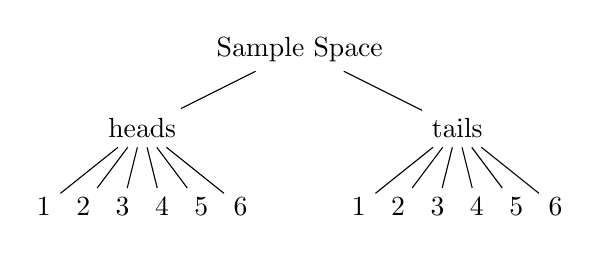
\begin{tikzpicture}
\node{Sample Space}
[level distance=1cm]
[sibling distance=.5cm]
	child {node{heads}
		child{node{1}}
		child{node{2}}
		child{node{3}}
		child{node{4}}
		child{node{5}}
		child{node{6}}}
child[missing]
child[missing]
child[missing]
child[missing]
child[missing]
child[missing]
child[missing]
	child {node{tails}
		child{node{1}}
		child{node{2}}
		child{node{3}}
		child{node{4}}
		child{node{5}}
		child{node{6}}};
\end{tikzpicture}
\end{center}

\noindent or alternatively

\begin{center}
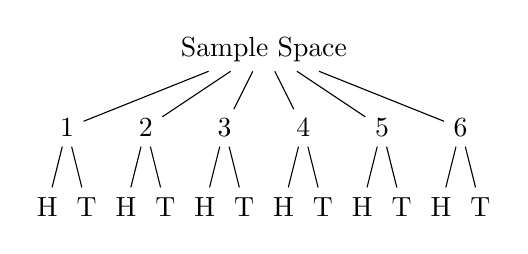
\begin{tikzpicture}
\node{Sample Space}
[level distance=1cm]
[sibling distance=.5cm]
	child {node{1}
		child{node{H}}
		child{node{T}}}
child[missing]
	child {node{2}
		child{node{H}}
		child{node{T}}}
child[missing]
	child {node{3}
		child{node{H}}
		child{node{T}}}
child[missing]
	child {node{4}
		child{node{H}}
		child{node{T}}}
child[missing]
	child {node{5}
		child{node{H}}
		child{node{T}}}
child[missing]
	child {node{6}
		child{node{H}}
		child{node{T}}};
\end{tikzpicture}
\end{center}

\noindent either way, they both imply
$$\Omega = \Big\{  (H,1), (H,2), (H,3), (H,4), (H,5), (H,6),$$
$$  (T,1), (T,2), (T,3), (T,4), (T,5), (T,6), \Big\}  $$

Or by definition of cartesian products, we can say, \\$~~\Omega = \{H,T\} \times \{ 1,2,3,4,5,6 \}$.\footnote{Recall: The definition of cartisian product is that its an ordered pair, not an unordered set. So our graph must reflect that.} Which we know we can graph, at least for cartisian products of 3 or less sets \\(usually only for 2).



\begin{center}
\begin{tikzpicture}
\draw[->] (-1,0) -- (6,0) 
node[right] {$Coin~Toss$}; 
\draw[->] (0,-1) -- (0,7) 
node[above] {$Die~Toss$}; 

\foreach \y in {1,2,3,4,5,6}
	\draw [shift={(0,\y)}, color=black] (2pt,0pt) -- (-2pt,0pt) node[left] {$\y$};

\draw [shift={(2,0)}, color=black] (0pt,2pt) -- (0pt,-2pt) node [below] {$H$};
\draw [shift={(4,0)}, color=black] (0pt,2pt) -- (0pt,-2pt) node [below] {$T$};

\coordinate (A) at (2,1);
\filldraw (A) circle (2pt);

\coordinate (A) at (2,2);
\filldraw (A) circle (2pt);

\coordinate (A) at (2,3);
\filldraw (A) circle (2pt);

\coordinate (A) at (2,4);
\filldraw (A) circle (2pt);

\coordinate (A) at (2,5);
\filldraw (A) circle (2pt);

\coordinate (A) at (2,6);
\filldraw (A) circle (2pt);

\coordinate (A) at (4,1);
\filldraw (A) circle (2pt);

\coordinate (A) at (4,2);
\filldraw (A) circle (2pt);

\coordinate (A) at (4,3);
\filldraw (A) circle (2pt) node[right] {$(T,3)$};

\coordinate (A) at (4,4);
\filldraw (A) circle (2pt);

\coordinate (A) at (4,5);
\filldraw (A) circle (2pt);

\coordinate (A) at (4,6);
\filldraw (A) circle (2pt);
\end{tikzpicture}
\end{center}








\subsection{Set Theory Examples}
%%%------------------- Lecture 2: 1/20/23
\textbf{Exercise B.4.} Show that identity the "de Morgan" Law, $$\left( \bigcap\limits_i A_i\right)^{C}=\bigcup\limits_i A_i^{C}$$ is true.\\

\noindent\textit{Recall:} We need to show that the LHS and RHS are subsets of eachother.\\ 
Similar to ``if and only if", however instead of \textbf{saying} 
\begin{itemize}
\item ``if $\rightarrow$ then... 
\item Conversely $\leftarrow$ then... 
\item Therefore $\iff{}$..." 
\end{itemize}

\noindent For set theory, we would \textbf{check} (for proper subsets btw), 
\begin{itemize}
\item $\subseteq :~~~$``Let $a \in A$, check that $a \in B$... yes! So since $a$ started in $A$, but is also in $B$, hence $A\subseteq B$"
\item $\supseteq :~~~$``\textbf{Now} (not conversely), let $b \in B$, check that $b \in B$... yes! So since $b$ started in $B$, but is also in $A$, hence $B\subseteq A$"
\item $=: ~~~$ Therefore since $\subseteq$ and $\supseteq$, then $A=B$.
\end{itemize}
Now that we remember this,\\

\noindent \textit{Proof by Professor:} ``$\subseteq$" direction first.

\noindent Let $x \in \left( \bigcap\limits_i A_i\right)^{C}$. \\

$\implies x \notin A_i=\{y~|~ y\in A_i,~\forall i\}$.\\

\noindent Then $\exists i~s.t.~ x\notin A_i$.\\
So $x \in \bigcup\limits_i A_i^{C}$\\
Hence, $\left( \bigcap\limits_i A_i\right)^{C}   \subseteq  \bigcup\limits_i A_i^{C}.$\\

\noindent"$\subseteq$" direction now.\\

\noindent Now let $x \in \bigcup\limits_i A_i^{C}$. \\
Then $x \in A_i^{C}$, for some $i\in \mathbb{Z}$.\\
Then $x \notin A_i$, for some $i\in \mathbb{Z}$.\\
Then $x \notin \bigcap\limits_i A_i \implies x\in \left( \bigcap\limits_i A_i\right)^{C}$,\\
Hence, $\bigcup\limits_i A_i^{C} \subseteq \left( \bigcap\limits_i A_i\right)^{C}$.\\

Therefore, \\
$$\left( \bigcap\limits_i A_i\right)^{C}=\bigcup\limits_i A_i^{C}$$\hfill$q.e.d.$\\


\noindent \textbf{Exercise B.5.} If $A$ and $B$ are sets then let $A triangle B$ denote their symmetric difference: the set of elements that are in exactly one of the two sets. (In words this is “$A$ or $B$, but not both.”) Prove that the symmetric difference is associative.\\

\noindent \textbf{Solution not Proof :)} \\
\indent We then go over B.5. however he goes over it with a proof by venn diagram. Which is somewhat trivial, and does not require much explanation/studying (which is why I dont really consider it a proof). \textit{no figure here}
However this is similar to doing proofs by table and I dislike this. But this is one of the few times I'll say, the proof is left as an exercise to the reader.\footnote{I am aware (and not naive...I think), that prooving this properly would take ~10 pages and 5 hours (not actually).}

Actually, since I'm stubborn $+$ I'm a nerd $=$ Hard way
Both are direct proofs.

\noindent \textit{Proof by Internet}\\
Similar to the venn diagram, we know\\
$(A \triangle B) \triangle C = (A \cup B \cup C) \cap (A \cup B^{C} \cup C^{C}) \cap (A^{C} \cup B \cup C^{C}) \cap (A^{C} \cup B^{C} \cup C)$\\
$= (B \cup C \cup A) \cap (B \cup C^{C} \cup A^{C}) \cap (B^{C} \cup C \cup A^{C}) \cap (B^{C} \cup C^{C} \cup A)$\\
$=(B \triangle C) \triangle A$.\\

Now, $\triangle$ is commutative since by $def^n$, obviously \\
$A\triangle B=(A\cap B^{C}) \cup (B \cap A^{C})= (B \cap A^{C}) \cup (A\cap B^{C}) = B\triangle A$.\\
\noindent So $(B \triangle C) \triangle A = A \triangle (B \triangle C)$.\hfill$q.e.d.$\\

\noindent \textit{Proof by Stubborness}\\
\noindent Notice $A\triangle B=(A\cap B^{C}) \cup (B \cap A^{C})$.\\

\noindent Then \\
$(A \triangle B) \triangle C = ((A \triangle B)\cap C^{C}) \cup (C \cap (A \triangle B)^{C})$\\
$=(((A\cap B^{C}) \cup (B \cap A^{C}))\cap C^{C}) \cup (C \cap ((A\cap B^{C}) \cup (B \cap A^{C}))^{C})$\\

\noindent Recall the De Morgan's law, $(A \cap B)^{C}= A^{C} \cup B^{C}$ and $(A \cup B)^{C}= A^{C} \cap B^{C}$\\

\noindent So, \\
$(((A\cap B^{C}) \cup (B \cap A^{C}))\cap C^{C}) \cup (C \cap ((A\cap B^{C}) \cup (B \cap A^{C}))^{C})$\\
$=(((A\cap B^{C}) \cup (B \cap A^{C}))\cap C^{C}) \cup (C \cap (A\cap B^{C})^{C} \cap (B \cap A^{C})^{C})$\\
$=(((A\cap B^{C}) \cup (B \cap A^{C}))\cap C^{C}) \cup (C \cap A^f{C} \cup B \cap B^{C} \cup A)$\\

\noindent ... yeah so I give up on this, I'll link a note on this when I find a clever but complete solution. Now that I have officially wasted 30 minutes of my saturday...\qed\\





\section{Random Sampling }
\subsection{Population and Sample Size}

\textbf{Some notation.}
Simply put, 
\begin{itemize}
\item Population Set: What we've been calling the sample space.
	\begin{itemize}\item``Population Size" $\# \Omega = n$.\end{itemize}
\item Sample Set: What we've been calling an event.
	\begin{itemize}\item``Sample Size" $\# A = k$, where $A$ is an event from the ``event space".\end{itemize}
\end{itemize}

I believe our professor is changing the terminology since it's more used or more practical, and less mathematical with its measure theory roots.

Main takeaways being, sample space $\neq$ sample set. They're different things, not related.

Also, we may still use $\Omega$ for both ``Sample Space" and ``Population Set".
As well as $\mathcal{F}$ for the ``Event Space" and ``Sample Size".
But more efficiently: I've been using the cardinality of these sets to denote the number of elements. But to step away from set theory, the textbook and other places use $\#$ instead.\\

\noindent \textbf{Quick example.}\\
Let the ``Population Set" $\Omega=\{a,b,c,d\}$,\\
then the ``Population Size" $\# \Omega = n = 4$.\\

\noindent Let our ``sample" be this event $A = \{b,d\}$,\\
then the ``sample size" $\# A = k = 2$.\\

\noindent \textbf{How Many Samples are there?}\\
This is our next important question. \\
--- How many samples are there given a population set, \\
or \\
--- rather how many events are there from a sample space.\\

\noindent \textit{Remark.} This question is kind of ambiguous, as I am not asking amount of all events in the ``event space" which would be the full set of all events (i.e. the cardinality of the power set). I am talking about what is the number of all the events if we have restrictions on \textit{how} we sample. 

So what are the restrictions/``procedures" we can do when making an event from a sample space. Well we can,
\begin{enumerate}
\item Sample with replacement, order matters := $n^k$
\item Sampling without replacement, order matters := \\$nPk = \frac{n!}{(n-k)!}$
\item Sample without replacement, order doesn't matter := $nCk = {n \choose k} = \frac{n!}{k!(n-k)!}$
\item Sample with replacement, order doesn't matter := \\${k+n-1 \choose n-1}={k+n-1 \choose k}$ 
\end{enumerate}

All of these are somewhat explanatory, increasing in complexity.

Also similarly, finding out (the amount of events) or (the different ways), we can sample goes from simple to complex as well.

But I'll try to walk through each logically, as well as proof wise, and I'll derive the formulas for finding out the number of possible samples/events.





\subsection{Sampling with replacement, \\order matters}
Suppose we have a sample space with $n$ elemtents. \\
--- I have a bag of $n=15$ marbles. They are colored.\\
Now suppose we want to take a sample of size $k$. \\
--- I want to pick $k=4$ marbles.\\

\noindent Let's choose: \\
We want the order to matter, so we will pick up one at a time, and record it.
\begin{itemize}
\item I grab 1 marble, its red. (then I mark it down)
\end{itemize}
We want the to sample \textbf{with} replacement, so after we pick one, we put it back in the bag.\\
--- I'll put this back in the bag (so theres a chance I could pick it again).

\noindent Then we repeat until we get our full sample (of size $k$).
\begin{itemize}
\item I grab 1 marble, its blue. (I mark it down) Ok, I'll put it back.
\item I grab 1 marble, its red. (I mark it down) Ok, I'll put it back. 
\item I grab 1 marble, its clear. (I mark it down) Ok, I'll put it back.
\end{itemize}
Thats what sampling with replacement looks like. \\
--- Overall: I have a bag of 15 marbles, and my sample was ``I chose 4 marbles". 

In this scenario, Imma put back the marbles each time (so I could get the same one each time). Also in this scenario, I care about the order. \\
--- So this time I got $\omega =$(red, blue, red, clear).\\

\noindent \textbf{How many outcomes are there? Logically.}\\
Well, simply put:\\
The first marble has $n$ posibilities. \\
The second marble has $n$ posibilities.\\
The third marble has $n$ posibilities.\\
The...$~~~~~~~~~~~~~~~~~~~~~$...posibilities.\\
$\downarrow ~~~~~~~~~~~~~~~~~~~~~~~~~~~~~~~~~~\downarrow$\\
The $k$th marble nas $n$ posibilities.

This is because we're sample with replacement, \\
i.e. each time I choose a marble, I put it back in the bag,\\
so I always have 15 marbles in the bag, so 15 posibilities.

So we have $$n*n*n*n*\cdots *n = n^k$$
$$k~~~times$$
And the number of outcomes is $$\#\Omega = n^k~.~~~\square$$

\noindent \textbf{How many outcomes are there? Proof wise.} \\
\textit{Proof.}
Let $S=\{1,2,...,n\}~for~some~n\in \mathbb{N}$.\\
Set an element of our sample space $\omega \in \Omega$ to be an ordered $k$-tuple of elements $s_i \in S.$\\
So $\omega = (s_1, s_2, s_3,..., s_k), ~for~some~k\in \mathbb{N}$.\\
Then 
$$\Omega = \big\{ (s_1, s_2, ..., s_k)_{k\in \mathbb{N}} ~\big|~ s_i \in S, ~i=1,2,...k \big\}$$
but this implies
$$ \Omega = S \times S \times \cdots \times S, ~k~times.$$
So therefore
$$ \#\Omega = \prod\limits_{i=1}^k S_i = n^k,~for~some~k\in\mathbb{N}.\footnote{Also quickly note, the probability measure (probability), if each event/outcome is equally likely implies 
$$P(\omega)=\frac{1}{\#\Omega} = n^{-k}~.~~~\square$$}$$\hfill$q.e.d.$




\subsection{Sampling without replacement,\\ order matters}
Suppose we have a sample space with $n$ elemtents. \\
--- I have a bag of $n=15$ marbles. They are colored.\\
Now suppose we want to take a sample of size $k$. \\
--- I want to pick $k=4$ marbles.\\

\noindent Let's choose: \\
We want the order to matter, so we will pick up one at a time, and record it.
\begin{itemize}
\item I grab 1 marble, its red.
\end{itemize}
This time, we sample \textbf{without} replacement, so after we pick one, we keep it and don't put it in the bag. \\
--- I put this on a rack, now the bag has $n-1=15-1=14$ marbles left.

\noindent Then we repeat until we get our full sample (of size $k$). 
\begin{itemize}
\item I grab 1 marble, its blue. Ok, I'll put it on the 2nd position on my rack. Now theres $n-2=15-2=13$ marbles left.
\item I grab 1 marble, its red. Ok, I'll put it on the 3nd position on my rack. Now theres $n-3=15-3=12$ marbles left.
\item I grab 1 marble, its clear. Ok, I'll put it on the 4nd position on my rack. Now theres $n-4=15-4=11$ marbles left.
\end{itemize}
Thats what sampling with replacement looks like. \\
--- Overall: I have a bag of 15 marbles, and my sample was ``I chose 4 marbles". 

In this scenario, keep the marbles in a rack, in order. (each time, theres 1 less marble, noting that i can only do this a max of $n=15$ times).\\
--- So this time I got $\omega =$(red, blue, red, clear).\\

\noindent \textbf{How many outcomes are there? Logically.} \\
Well, simply put:\\
The first marble has $n$ posibilities. \\
The second marble has $n-1$ posibilities.\\
The third marble has $n-2$ posibilities.\\
The...$~~~~~~~~~~~~~~~~~~~~~~~~$...posibilities.\\
$\downarrow ~~~~~~~~~~~~~~~~~~~~~~~~~~~~~~~~~~~\downarrow$\\
The $k$th marble nas $n-k$ posibilities, noting that $k\ngtr n$ since you can't pick up more than n marbles. \\
This does imply that the $k$th marble has only 1 posibility if instead $k\geq n$, so we should say it has $(n-k) + 1$ posibility.

So we have $$n*(n-1)*(n-2)* \cdots *(n-k+1) = nPk.$$
Where we say $nPk$ is the number of $k$ permutations of $n$.

The number of outcomes is easier to calculate if we rewrite this formula as...
$$\#\Omega = nPk = \frac{n!}{(n-k)!}$$
since 
$$n*(n-1)*(n-2)* \cdots *(n-k+1)$$
$$ = \frac{n!}{(n-k)(n-k-1)(n-k-2)\cdots 3*2*1}.~~~\square$$

\noindent \textbf{How many outcomes are there? Proof wise.}\\
\textit{Proof.}
Let $S=\{1,2,...,n\}~for~some~n\in \mathbb{N}$.\\
Set an element of our sample space $\omega \in \Omega$ to be an ordered $k$-tuple of elements $s_i \in S$.\\
So $\omega = (s_1, s_2, s_3,..., s_k), ~for~some~k\in \mathbb{N}$.\\
But this time this tuple has elements $s_i\in S$,  that are distinct. So, $s_i \neq s_j, ~\forall i\neq j.$\\
Then \\
$$\Omega = \big\{ (s_1, s_2, ..., s_k)_{k\in \mathbb{N}} ~\big|~ s_i \in S, s_i \neq s_j, ~\forall i\neq j. \big\}$$
but this implies
$$n*(n-1)*(n-2)* \cdots *(n-k+1) = nPk$$
$$\textstyle =n*(n-1)*(n-2)* \cdots *(n-k+1)*\frac{(n-k)(n-k-1)(n-k-2) *\cdots *3*2*1}{(n-k)(n-k-1)(n-k-2) *\cdots *3*2*1}$$
$$\textstyle =\frac{n*(n-1)*(n-2)* \cdots *(n-k+1)(n-k)(n-k-1)(n-k-2) *\cdots *3*2*1}{(n-k)(n-k-1)(n-k-2) *\cdots *3*2*1}$$
$$=\frac{n!}{(n-k)!}.$$
So therefore
$$ \#\Omega = nPk = \frac{n!}{(n-k)!}.$$\hfill$q.e.d.$




\subsection{Sampling without replacement, \\ order doesn't matter}
Suppose we have a sample space with $n$ elemtents. \\
--- I have a bag of $n=15$ marbles. They are colored.\\
Now suppose we want to take a sample of size $k$. \\
--- I want to pick $k=4$ marbles.\\

\noindent Let's choose: \\
We don't care about order, so we will just hold it in our hand.
\begin{itemize}
\item I grab 1 marble, its red. It is in my hand.
\end{itemize}
We are not sampling with replacement, so after we pick one I pick up another one and keep it in my hand.
\begin{itemize}
\item I grab 1 marble, its blue. Ok, I'll keep this in my hand.
\end{itemize}
Then we repeat until we get our full sample (of size $k$). 
\begin{itemize}
\item I grab 1 marble, its red. Ok, I keep this in my hand.
\item I grab 1 marble, its clear. Ok, I keep this in my hand.
\end{itemize}
Thats what sampling with replacement looks like. \\
--- Overall: I have a bag of 15 marbles, and my sample was ``I chose 4 marbles". 

In this scenario, Imma put back the marbles each time (so I could get the same one each time). Also in this scenario, I care about the order. \\
--- So this time I got the \textbf{set} $\omega =\big\{2~red's, blue, clear\big\}$ in my hand.\\

\noindent \textbf{How many outcomes are there? Logically.} \\
Well, simply put:\\
The first marble has $n$ posibilities. \\
The second marble has $n-1$ posibilities.\\
The third marble has $n-2$ posibilities.\\
The...$~~~~~~~~~~~~~~~~~~~~~~~~$...posibilities.\\
$\downarrow ~~~~~~~~~~~~~~~~~~~~~~~~~~~~~~~~~~~\downarrow$\\
The $k$th marble nas $n-k$ posibilities, noting that $k\ngtr n$ since you can't pick up more than n marbles. \\
This does imply that the $k$th marble has only 1 posibility if instead $k\geq n$, so we should say it has $(n-k) + 1$ posibility.

So we have $$n*(n-1)*(n-2)* \cdots *(n-k+1).$$

The number of outcomes is easier to calculate if we rewrite this formula as...
$$\#\Omega = nPk = \frac{n!}{(n-k)!}$$
since 
$$n*(n-1)*(n-2)* \cdots *(n-k+1)$$
$$ = \frac{n!}{(n-k)(n-k-1)(n-k-2)\cdots 3*2*1}.$$

Now lastly note that for each event $\omega$, it is a proper subset of S. Also this is not an ordered $k$-tuple. So each $\omega$ can be rearranged in many ways. I.E. The permutations do not matter, what we care about is the \textbf{combinations}.

We can kind of cheat and make this simpler, since we are only picking up $k$ amount, we don't have to consider all of the possible unordered subsets, just the $k$ amount of subsets we pick. Each subset can be rearranged in $k!$ ways. So out ot the $n!$ posibilities, the $(n-k)!k! \implies (n-k)!k!$.

\noindent And so, 
$$\#\Omega = \frac{n!}{(n-k)!k!} = nCk ={n \choose k},$$
which makes sense since $nPa \geq nCk.~~~\square$\\
--- Read: ``$n$ choose $k$"

\noindent \textbf{How many outcomes are there? Proof wise.}\\
\textit{Proof.}
Let $S=\{1,2,...,n\}~for~some~n\in \mathbb{N}$.\\
Set an element of our sample space $\omega \in \Omega$ to be an unordered set with elements $s_i\in S$. Since we are going without replacement, the amount of elements in each subset have to add up to the total amount of elements in our sample space, i.e. $\sum (\#s_i \in  \omega _i) = \#\Omega$. But this also imples that all $\omega_i$ are proper subsets of S. \\
So $$\Omega = \big\{  \omega \subset S ~\big|~ \# = k,~1\leq k \leq n  \big\}.$$
Now we know for the amount of permutations of $\Omega$ is,
$$ \#\Omega = nPk = \frac{n!}{(n-k)!}.$$
And the total amount of subsets $\omega$, has been counted $k!$ times. (first $k$ has been counted $k$ times = $k$ permutations). \\
So we need to delete this amount from our number of permutations formula\\
but this implies\\
$${nCk} ~\implies~{ \frac{nPk}{k!} = \frac{n*(n-1)*(n-2)* \cdots *(n-k+1)}{k!}}$$
which we know we can simplify to
$$nCk = \frac{n!}{k!(n-k)!}.$$\hfill$q.e.d.$





\subsection{Sampling with replacement,\\ order doesn't matter}
Suppose we have a sample space with $n$ elemtents. \\
--- I have a bag of $n=15$ marbles. They are colored.\\
Now suppose we want to take a sample of size $k$. \\
--- I want to pick $k=4$ marbles.\\

\noindent Let's choose: \\
We don't care about order, so we will just mark it down as a set/combination.
\begin{itemize}
\item I grab 1 marble, its red. Marked down 1 red.
\end{itemize}
We want the to sample with replacement, so after we pick one, we put it back in the bag. 
\begin{itemize}
\item I got one blue, I'll put this back in the bag (so theres a chance I could pick it again).
\end{itemize}
Then we repeat until we get our full sample (of size $k$). 
\begin{itemize}
\item I grab 1 marble, its red. Ok, I'll put it back. 
\item I grab 1 marble, its clear. Ok, I'll put it back.
\end{itemize}
That's what sampling with replacement looks like. \\
--- Overall: I have a bag of 15 marbles, and my sample was ``I chose 4 marbles". 

In this scenario, Imma put back the marbles each time (so I could get the same one each time). Also in this scenario, I care dont care about the order, just the combination.\\
--- So this time I got the \textbf{set} $\omega =\big\{2~red's, blue, clear\big\}$.

\noindent \textbf{How many outcomes are there? Logically.} \\
Well, simply put:\\
We want combinations of these, so we will use 
$$\Omega = {n \choose k} = \frac{n!}{k!(n-k)!}.$$
But this time, we can take any combination of each combination. So consider each combination's elements, $x_i \in \omega,$ (where $\omega= (x_1,x_2,x_3...x_i)$). 

Then what I am saying is that we can rearrange $x_i$ in many different ways. For simplicity sake (and by our professor's idea), consider using ``dividers". In this fasion, there are $k$ distinct samples from the $nCk$ equation. And for each sample we can then take each $x_i$ and split it into its components. \\
E.g. $x_1 = 2~red = 1~red+1~red = 0+2~red = 2~red+0,$ where in this case, we treat + as the divider.

Similarly, we can have a box of donuts, and there are ``$\infty$-many" choices (w/ replacement i.e. the same flavors), as well as the order doesn't matter, ``we got 3 chocolate, 4 strawberry, and 5 glazed". Then we can ``break down" each \\
$x_i = \{ 3~chocolate,~4~strawberry,~5~glazed \}$ into  \\
$x_i = \{ 1~chocolate,~ 1~chocolate,~ 1~chocolate,~1~strawberry,~ 1~strawberry,~\cdots ~1~glazed,~1~glazed,\}$\\
and then use dividers to split this into as many partitions as we would like.

Now how many dividers are there again?\\
Well each solution can be represented by $k$ elements, $x_1,...,x_k$.\\
And then there should be $n-1$ lines since there are only $n$ options (colors, flavors of donuts, etc.)

And the main idea is we can ``permute" these dividers whereever we like. To cheat though, we can just consider \textbf{all} the combinations of the sample points (colors/flavors) + all the dividers, compared to how many we pick ($k$ amount (which can be larger than the $\#\Omega$).

So finally our equation is 
$$ {n \choose k} \implies {[n + (k-1)] \choose k} = {n+k-1 \choose n-1}.~~~\square$$

\noindent \textbf{How many outcomes are there? Proof wise.}\\
\textit{Proof.}
Let $S=\{1,2,...,n\}~for~some~n\in \mathbb{N}$.\\
Set an element of our sample space $\omega \in \Omega$ to be an unordered set with elements $s_i\in S$. Since we are going without replacement, the amount of elements in each subset have to add up to the total amount of elements in our sample space, i.e. $\sum (\#s_i \in  \omega _i) = \#\Omega$. But this also imples that all $\omega_i$ are proper subsets of S. \\
So $$\Omega = \big\{  \omega \subset S ~\big|~ \# = k,~1\leq k \leq n  \big\}.$$
Now we know for the amount of permutations of $\Omega$ is,
$$ \#\Omega = nPk = \frac{n!}{(n-k)!}.$$
And the total amount of subsets $\omega$, has been counted $k!$ times. (first $k$ has been counted $k$ times = $k$ permutations). \\
So we need to delete this amount from our number of permutations formula\\
but this implies\\
$$nCk ~\implies{}~ \frac{nPa}{k!} = \frac{n*(n-1)*(n-2)* \cdots *(n-k+1)}{k!}$$
which we know we can simplify to
$$nCk = \frac{n!}{k!(n-k)!}.$$
Now, consider the elements of our sample space $\omega_i \in \Omega$.\\
Note that since $\omega\in \Omega$, then for $\omega \ni n_i \in S$.\\
But now we can partition $\omega$ and its $k$ elements $n_1,...,n_i,...n_k$, with $n-1$ disjoint unions.\\
This implies there are now $k + (n-1)$ "objects", which we can take any combination of. Where for each instance of two adjacent disjoint unions, we take the union of the empty set, i.e. $\cdots \dot{\cup}~\dot{\cup} \cdots = \cdots \dot{\cup}~\emptyset~\dot{\cup} \cdots.$\\
So then we have \\
$${n \choose k} \implies {[n + (k-1)] \choose k} \implies {n + k-1 \choose k}= {n+k-1 \choose n-1}. ~~~~~\blacksquare$$

Summary: Just Memorize
\begin{enumerate}
\item Sample with replacement, order matters := $n^k$
\item Sampling without replacement, order matters := \\$nPk = \frac{n!}{(n-k)!}$
\item Sample without replacement, order doesn't matter := $nCk = {n \choose k} = \frac{n!}{k!(n-k)!}$
\item Sample with replacement, order doesn't matter := \\${k+n-1 \choose n-1}={k+n-1 \choose k}$ 
\end{enumerate}
As well as, for grabbing marbles one by one...
\begin{enumerate}
\item Sampling with replacement $\implies{}$ putting marbles back into the bag
\item Sampling without replacement $\implies{}$ keeping the marbles out of the bag
\item Order matters $\implies{}$ put it in on a rack in order, or mark down the tuple (which came first) $\implies{}$ permutations
\item Order doesn't matter $\implies{}$ hold it in your hand, or mark down the set $\implies{}$ combinations
\end{enumerate}

\subsection{Random Sampling Examples}

\textbf{E.g. 1.8} Suppose a bag of scrabble tiles contains $5~E's,4~A's,$ \\$3~N's,$ and $2~B's$. Draw $4$ tiles without replacement.
\begin{itemize} \item[(a)] Find $P(C)$ by imagining that the tiles are drawn one by one, as an ordered sample.\end{itemize}
\textit{Solution.}
Let $C = \{ 2~E,~1~A,~1~N \}$. (Note sets are unordered)
Suppose you have
\begin{align*}
&P(1st~E,~2nd~E,~3rd~A,~4th~N)\\
&+ P(1st~E,~2nd~A,~3rd~E,~4th~N)\\
&+ P(1st~N,~2nd~A,~3rd~E,~4th~E) + \cdots
\end{align*}
$$ = \frac{(5*4)*(4)*(3)}{14*13*12*11} + \frac{(5*4)*(4)*(3)}{14*13*12*11} + \frac{(3)*(4)*(5)*(4)}{14*13*12*11}+\cdots$$
$$=\frac{5*4*4*3}{14*13*12*11} {4 \choose 2}{2\choose 1}{1\choose 1}$$
$$=\frac{5*4*4*3}{14*13*12*11} \left( \frac{4*3}{2*1} \right) \left( \frac{2*1}{1} \right) \left(\frac{1}{1}\right) \approx 0.0599. ~~~\square$$
\begin{itemize}\item[(b)] Find $P(C)$ by imaging that the tiles are drawn all at once as an unordered sample.\end{itemize}
Or more simply,
$$\frac{ {5\choose 2}{3\choose 1}{4\choose 1}  }{{14\choose 4}}.$$
which gives the same value, $\approx 0.059$.$~~~\square$\\

\noindent \textbf{E.g. 1.8} Everyday a kindergarten class chooses randomly one of the 50 state flags to hang on the wall, without regard to previous choices.
\begin{itemize}\item [(a)] Find the sample space.\end{itemize}
\textit{Solution.} Let $S=\{1,2,3,4,...,50\}$, then 
$$\Omega=S\times S\times S = \big\{(i,j,k) ~\big|~ i,j,k\in S \big\}.$$
and then $$\#\Omega = 50*50*50 = 50^3.~~~\square$$
\begin{itemize}\item [(c)] Find the probability that the Wisconsin flag will be hung at least two of the three days, Monday, Tuesday, and Wednesday.\end{itemize}
\textit{Solution.}\\
Lets seperate this into the probability of 2 days, and probability of 3 days (which includes 2).\\
$$P(W~W~else)+P(W~else~W)+P(else~W~W)+P(W~W~W) $$
$$= \frac{1*1*49}{50*50*50}*3+\frac{1*1*1}{50^3}.~~~\square$$

\newpage
\noindent \textbf{E.g. 1.13} Suppose we have a class of $24$ students.
\begin{itemize}\item [(a)] A team of three children is chosen at random. Find the probability that the team consists of Shane, Heather, and Laura.\end{itemize}
\textit{Solution.} \\
So we need to find 
$$P\big(\{Shane, ~Heather, ~Laura\}\big) = \frac{1}{{24 \choose 3}}.~~~\square$$
\begin{itemize}\item [(c)] Find the probability that Mary is on the team.\end{itemize}
\textit{Solution.} 
$$P\Big(\big\{ \{Shane, ~Heather, ~Laura\} \land \{Mary\} \big\}\Big) = \frac{{23\choose 2}}{{24\choose 3}}.~~~\square$$

\noindent \textbf{E.g. ?.?} Three students are chosen to be class president, vice president, and treasurer. No student can hold more than one office. \\
\begin{itemize}\item [(a)] Find the probability that mary is president, cory is vice president, and matt is treasurer.\end{itemize}
\textit{Solution.}\\
Let event $A$ be the event in part (a) holds. Then 
$$P(A) = \frac{1*1*1}{24*23*22}.~~~\square$$
\begin{itemize}\item [(b)] What is the probability that ben is either president or vice president.\end{itemize}
\textit{Solution.}\\
Let event $B$ be the event in part (b) holds. Then 
$$P(A) = \frac{1*23*22}{24*23*22} + \frac{23*1*22}{24*23*22} = \frac{1}{24}+\frac{1}{24} = \frac{1}{12}.~~~\square$$

%%%------------------------ Lecture 4: 1/25/23
\noindent \textbf{E.g. 1.7} We have an urn with 3 green and 4 yellow balls. We draw 3 one by one without replacement.
\begin{itemize}\item [(a)] Find the probability that the colors we see in order are green, yellow, green.\end{itemize}
\textit{Solution.} \\
Note: order matters, without replacement. So,
$$P(\omega) = \frac{3*4*5}{7*6*5}~.~~~\square$$
\begin{itemize}\item [(b)] Find the probability that our sample of 3 balls contain 2 green balls and 1 yellow ball.\end{itemize}
\textit{Solution.} \\
Note: order doesn't matter, without replacement. So,
$$P(\omega) = P (y,g,g) + P (g,y,g) + P(g,g,y)$$
$$=\frac{3*4*2}{7*6*5} + \frac{3*2*4}{7*6*5} + \frac{4*3*2}{7*6*5}$$
$$=\frac{3*4*2}{7*6*5} * {3 \choose 1} = \frac{3*4*2}{7*6*5} * 3 = \dfrac{{3\choose 2}{4\choose 1}}{{7\choose3}}~.~~~\square$$

\noindent \textbf{E.g. 1.10} We roll a fair die repeatedly until we see the number four appear and then stop. The outcome of the expirement is the number of rolls.
\begin{itemize}\item [(a)] Find the sample space $\Omega$ and the probability measure $P$. \end{itemize}
\textit{Solution.} \\
The sample space goes on until infinity with discrete steps, so
$$ \Omega = \big\{ 1,2,3,4,... \big\} \cup \big\{ \infty \big\}.$$
Also our probability measure should be for a finite amount of trials, set this amount to be ``$k$-trials". Then\footnote{Technnically, we should define a probability measure using the definition. So for and event that is also $A\subseteq \Omega$, we set $P(A)=\sum\limits_{k\in A} P(A)$.},
$$ P(k) = \frac{5^{k-1}*1}{6^k}.~~~\blacksquare$$
\begin{itemize}\item [(b)] Calculate the probability that the number never appears.\end{itemize}
\textit{Solution.} \\
The probability that the number never appears implies the probability that there are infinite events.
Which is
$$P(\infty)=1-\sum\limits_{k=1}^{\infty} P(k) = 1- \sum\limits_{k=1}^{\infty} \frac{5^{k-1}}{6^k}$$
$$ = 1-\frac{a}{1-r} = 1-\frac{\frac{1}{6}}{1-\frac{5}{6}}$$
$$ = 1-\frac{\frac{1}{6}}{\frac{1}{6}} = 1-1 = 0.$$
So,\footnote{This such definition can be taken in a limit process as well, at least in this case. So you would set $\{\infty \} \subseteq \{F,F,F...,F\},$ of size $k$. Or better defined, $|\{F,F,F...,F\}|=k,~\forall k\in \mathbb{N}$. Then $P(\infty) \leq P(F...F) = \frac{5^k}{6^k} = \left( \frac{5}{6} \right)^k \rightarrow 0,$ as $k\rightarrow 0$. This is opposite to the probability I get a 100\% in this class, so at least I have that going for me.}
$$P(\infty) = 0.~~~\square$$






\section{Infinite many outcomes}
\hypertarget{infinitely many outcomes}{Key Idea:} infinite/uncountable sets $\implies{}$ probabilities are continuous over $\mathbb{R}$. ($\mathbb{R}$ is the new thing here). We shall look at some examples, it should be fairly simple.\\

\noindent \textbf{E.g. 1.16} Flip a coin until the first tails comes up. Record the number of flips required as the outcome of the experiment.\\
\begin{itemize} \item[(a)] Find the sample space.\end{itemize}
\textit{Solution.}
Then the sample space is  $$\Omega = \{1,2,3,...\}\cup \{\infty\}.~~~\square$$
\begin{itemize} \item[(b)] Find $P(k)$.\end{itemize}
\textit{Solution.}
Well, there are $n=2$ posibilities for each sample point.\\
The $k$th event can be described as the following,\\
$k=5 ~\implies~H*H*H*H*H*T.$\\
So $$P(k) = \frac{1*1*1*\cdots *1}{2^k}, ~for~k=1,2,3,...$$
And also 
$$P(\infty) = 1- \sum\limits_{k=1}^{\infty} P(k)= 1- \sum\limits_{k=1}^{\infty} \frac{1}{2^k},$$
which is a geometric series, with $a_1 = \frac{1}{2}$, common ratio $r=\frac{1}{2}$.\\
So since this one starts at $k=1$, 
$$1- \sum\limits_{k=1}^{\infty} \frac{1}{2^k} = 1-\frac{a}{1-r} = 1-\frac{\frac{1}{2}}{1-\frac{1}{2}}$$
$$=1-\frac{\frac{1}{2}}{\frac{1}{2}}=1-1 = 0.$$
So the probability that you never get tails/you keep getting heads, in this limit process of a \textbf{fair} coin, is 
$$P(\infty) = 0.~~~\square$$

\noindent \textbf{E.g. 1.17}- We pick a real number uniformly at random reom the closed interval $[0,1]$.\\
\begin{itemize} \item[(a)] Find the sample space. \end{itemize}
\textit{Solution.}
$$\Omega = \{a\in \mathbb{R} ~|~ 0\leq x \leq 1\} = [0,1].~~~\square$$
\begin{itemize} \item[(b)] Find $P\left(\frac{1}{2} \leq x \leq \frac{3}{4}\right)$\end{itemize}
\textit{Solution.}
$$P\left(\frac{1}{2} \leq x \leq \frac{3}{4}\right) = \frac{\frac{3}{4} - \frac{1}{2}}{1} = \frac{1}{4}.~~~\square$$

\noindent \textbf{E.g. 1.18} - Consider a dartboard in the shape of a disk with radius of 9 inches. The bullseye is a disk of diameter $\frac{1}{2}$ inch in the middle of the board. What is the probability that a dart randomly thrown on the board hits the bullseye?\\
\textit{Solution.}
$$P(hitting~the~bullseye) = \frac{Area(bullseye)}{Total~area}$$
$$ = \frac{\pi \left( \frac{1}{9} \right)^2}{\pi (9)^2} = \frac{\frac{1}{16}}{81} = \frac{1}{(16)(81)}.~~~\square$$




%%%--------------------- Lecture 5: 1/30/23
\section{Consequences of \\the Rules of Probability} 
These are the three main properties that come from the Rules of Probability (i.e. the way we had described and defined our $\sigma$-algebra "$P(A),A\in\mathcal{F}=|\Omega|$" and Probability Space)
\begin{enumerate}
\item Decomposition of an event.
\begin{itemize} \item If $A = \bigcup\limits_{i=1}^\infty A_i$, where $A_1,A_2,...$ are pairwise disjoint events, then $P(A) = \sum\limits_{i=1}^\infty P(A_i)$.\end{itemize}
\item Events and Complements
	\begin{itemize} 
		\item $P(A)+P(A^C)=1$
		\item $P(A^C)=1-P(A)$
	\end{itemize}
\item Monotonicity of Probability
\begin{itemize} \item If $A\subseteq B,$ then $P(A)\subseteq P(B)$.\end{itemize}
\end{enumerate}
Below we will give examples and prove some of these consequences.

\subsection{Decomposing an event}
If $A = \bigcup\limits_{i=1}^\infty A_i$, where $A_1,A_2,...$ are pairwise disjoint events, then $P(A) = \sum\limits_{i=1}^\infty P(A_i)$

\noindent \textbf{E.g. 1.19} Suppose an urn contains 30 red, 20 green and 10 yellow balls. Draw two without replacement. What is the probability that the sample contains exactly one red or exactly one yellow?\\ 
\textit{Solution}\\
So the question is asking, $P(exactly~1~red~or~exactly~1~yellow)$.\\
\textbf{Main question:} Can you decompose this into other probabilities?\\
Without replacement $\implies{}$  means all the events can be broken up into disjoint unions. So therefore its probabilities can also be broken up.\footnote{You have to be very careful when you can or can't do this. }\\
\textbf{Ans:} Yes you can! i.e.\\
$P(exactly~1~red~or~exactly~1~yellow)$\\

$= P\big(   ~\{1r,1y\} \cup \{1r,1g\} \cup \{1y,1g\}~   \big)$\\

$=P\big(  \{1r,1y\}  \big) + P\big(  \{1r,1g\}  \big) + P\big(  \{1y,1g\}  \big)$\\

$=\dfrac{{30\choose1}{10\choose1}}{{60\choose2}} + \dfrac{{10\choose1}{20\choose1}}{{60\choose2}} + \dfrac{{30\choose1}{20\choose1}}{{60\choose2}}$\\

$=\dfrac{{30\choose1}{10\choose1}+{10\choose1}{20\choose1}+{30\choose1}{20\choose1}}{{60\choose2}}$\\

$=\dfrac{30*10+10*20+30*20}{\frac{60!}{2!*58!}}$\\

$= \dfrac{300+200+600}{    \frac   {\cancelto{30}{60} *59*\cancel{58!}}  {\cancelto{1}{2} *\cancel{58!}    }      }$ \\

$= \dfrac{1100}{30*59} = \dfrac{550}{15*59} = \dfrac{110}{3*59}=\dfrac{110}{117}.~~~\blacksquare$\\

\noindent \textbf{Recall} If $A_{1},A_{2}, ...$ are pairwise disjoint events, then $$P\left(\bigcup\limits_{i=1}^{\infty}A_{i}\right) = \sum\limits_{i=1}^{\infty}P(A_{i}).$$

\newpage
\noindent \textbf{E.g. 1.20} Peter and Mary take turns rolling a fair die. If Peter rolls 1 or 2 he wins and the game stops. If Mary rolls 3, 4, 5, or 6, she wins and the game stops. They keep rolling in turn until one of them wins. Suppose Peter rolls first.
\begin{itemize}\item [(a)] What is the probability that Peter wins and rolls at most 4 times?\end{itemize}
\textit{Solution.} 
Let $A_i=\{Peter~wins~at~his~i^{th}~roll\}$\\
Say the game looks like this...\\
I order it as ``step number, the player, if they win or not, and probability that they would have won"\\
$$\begin{aligned}
1.~Peter : F : \frac{4}{6}\\
2.~Mary : F : \frac{2}{6}\\
3.~Peter : F : \frac{4}{6}\\
4.~Mary : F : \frac{2}{6}\\
.\\
.\\
.\\
(i).~Peter : T : \frac{4}{6}\\
\end{aligned} $$
Then 
\begin{align*}
&P(Peter~wins~and~rolls~at~most~4~times)\\\\
&=P(A_{1}) + P(A_{2}) + P(A_{3}) + P(A_{4}) \\\\
\end{align*}
\begin{align*}
&=\displaystyle\sum\limits_{i=1}^{4} \left(\frac{4}{6}* \frac{2}{6}\right)^{i-1} \left(\frac{2}{6}\right)\\\\
&=\frac{1}{3}\sum\limits_{i=1}^{4} \left(\frac{2}{9}\right)^{i-1}\\\\
&=\frac{1}{3} \left[ \left(\frac{2}{9}\right)^{0} + \left(\frac{2}{9}\right)^{1}+ \left(\frac{2}{9}\right)^{2} + \left(\frac{2}{9}\right)^{3} \right] \\\\
&=\frac{1}{3} \left[ \frac{1}{3} + \frac{2}{9} + \left(\frac{2}{9}\right)^{2} + \left(\frac{2}{9}\right)^{3} \right] \\\\
&=\frac{1}{3} ~~\dfrac{1-\left(\dfrac{2}{9}\right)^{4}}{1-\left(\dfrac{2}{9}\right)} \approx 0.427~~~\square
\end{align*}
\begin{itemize}\item [(b)] What is the probability that May wins?\end{itemize}
\textit{Solution.}
Let $B_i=\{Mary~wins~at~her~i^{th}~roll\}$\\
Say the game looks like this...\\
$$\begin{aligned}
1.~Peter : F : \frac{4}{6}\\
2.~Mary : F : \frac{2}{6}\\
\end{aligned} $$
$$\begin{aligned}
3.~Peter : F : \frac{4}{6}\\
4.~Mary : F : \frac{2}{6}\\
.\\
.\\
.\\
\end{aligned} $$
Then 
$$
\begin{aligned}
P(Mary~Wins)&=\sum\limits_{i=1}^{\infty} P(B_{i})\\\\
&= \sum\limits_{i=1}^{\infty} \left[ \left(\frac{4}{6}\right) \left(\frac{2}{6}\right) \right]^{i-1} \left(\frac{4}{6}\right)\\\\
&=\sum\limits_{i=1}^{\infty} \left(\frac{2}{9}\right)^{i-1} \left(\frac{2}{3}\right)\\\\
&= \left(\frac{2}{3}\right)^{2} \frac{a}{1-r}\\\\
&=\left(\frac{2}{3}\right)^{2} \frac{1}{1-\frac{2}{9}}\\
&=\left(\frac{2}{3}\right)^{2} \left(\frac{9}{7}\right) = \frac{4}{7} \approx 0.571~~~\square
\end{aligned}
$$




\newpage
\subsection{Events and Complements}
Both shall hold, 
\begin{itemize}
\item $P(A)+P(A^C)=1$
\item $P(A^C)=1-P(A)$
\end{itemize}

\noindent \textbf{E.g. 1.21} Roll a fair die 4 times. What is the probability that some numbers appears more than once?\\
\textit{Solution.}
$$
\begin{aligned}
&P(some~\#'s~appear~more~than~once)\\\\
&=1-P(all~numbers~are~different)\\\\
&=1-\frac{\cancel{6}*5*\cancelto{\cancel{2}}{4}*\cancel{3}}{\cancel{6}*6*\cancelto{3}{6}*\cancelto{\cancel{2}}{6}}\\\\
&=1-\frac{5}{18} = \frac{13}{18}=.722~~~\square
\end{aligned}
$$




\subsection{Monotonicity of Probability}
\textbf{Claim:} If $A\subseteq B,$ then $P(A)\subseteq P(B)$.\\
\textit{Proof.} 
Let $A,B$ be sets in $\Omega$.
Suppose $A\subset B$.\\
Then $B=A~\dot{\cup}~(B\backslash A)$\\
($\dot{\cup}$ meaning disjoint union).\\
Since this is a disjoint union, we can take the individual probabilities.\\
So,\\
$P(B)=P(A)+P(B\backslash A) \geq P(A) +0 =P(A)$\hfill $q.e.d.$\\

\noindent \textbf{E.g. 1.22} Suppose we toss a fair coin repeatedly. What is the probability that tails never occurs?\\
\textit{Recall.} We know $P(tails~never~occur)=0$ \hyperlink{infinitely many outcomes}{already}. This is by using a a summation generalized to $k$, and as it approaches $\infty$, we find $P(A)\to 0$.\\
However lets prove this using the new property ``Monotonicity of Probability" and the squeeze theorem.\\

\noindent \textit{Solution.} 
We know
\begin{align*}
0&\leq P(tails~never~occur) \\
&\leq P(tails~never~occur~in~the~1st~k~tosses)\\
&=\left(\frac{1}{2}\right)^{k},~\forall k\in \mathbb{N}.\\
\end{align*}
Then by the right hand side inequality, you may see, how the squeeze theorem will be used. Also the ratio $\left(\dfrac{1}{2}\right)^{k}$ is because each $k$th flip has a probability measure of $\frac{1}{2}$.\\
So now 
$$\lim\limits_{k\to \infty} \left(\frac{1}{2}\right)^{k}=0$$
or alternatively 
$$P(tails~never~occur~in~the~1st~k~tosses)=\left(\frac{1}{2}\right)^{k} ~\xrightarrow{k\to \infty}~0.$$
And by the squeeze theorem (from Calculus)
$$P(tails~never~occur)=0.$$\hfill$q.e.d.$

\newpage
\noindent \textbf{Question:} What if the probability measure was not fair?\\
Say a coin wasn't fair and had probability measures\\
$P(\omega) \neq P(H)=P(T)$, and we set\\
$P(H)=0.99 \implies P(T) = 0.01$.\\
But then, like the previous example, we get the same results, since by squeeze theorem
$$\begin{aligned}
0\leq &P(tails~never~occur) \\\leq 
&P(tails~never~occur~in~the~1st~k~tosses)\\
&=\left(0.99\right)^{k} ~\xrightarrow{k\to \infty}~ 0 
,~\forall k\in \mathbb{N}.
\end{aligned}$$



%%%---------------------------- Lecture 6: 2/1/23
\subsection{More Examples of these Consequences}
\noindent \textbf{E.g. 1.15} - An urn contains 4 balls: 1 white, 1 green, and 2 red. We draw 3 balls \textit{with} replacement. Find the probability that we \textit{did not} see all three colors.
\begin{itemize}\item[(a)] Solve with Inclusion-Exclusion Principle.\end{itemize}
\textit{Solution.}\\
Let $W = \{white~ball~did~not~appear\}$, \\
$G = \{green~ball~did~not~appear\}$, and \\
$R = \{red~ball~did~not~appear\}$.\\
Then 
\begin{align*}
&P\{we~did~see~all~three~colors\} \\\\
&= P(W \cup G \cup R) \\\\
&=P(W) + P(G) + P(R)\\
&P(W \cap G) -P(W \cap R) -P(G \cap R)\\
&+P(W\cap G\cap R)\\\\
\end{align*}

\begin{align*}
&=\frac{3*3*3}{4*4*4} + \frac{3*3*3}{4*4*4} + \frac{2*2*2}{4*4*4}\\
&-\frac{2*2*2}{4*4*4} - \frac{1*1*1}{4*4*4} - \frac{1*1*1}{4*4*4}\\
&+\frac{0*0*0}{4*4*4}\\\\
&=\frac{3^{3}+3^{3}-1-1}{4^{3}}=\frac{52}{64} = \frac{26}{32} = \frac{13}{16}.~~~\square
\end{align*}
\begin{itemize}\item[(b)] Solve using the complement.\end{itemize}
\textit{Solution.}\\
\begin{align*}
&P\{we~did~see~all~three~colors\}\\\\
&=1-P(we~saw~all~three~colors)\\\\
&=1- \frac{1*1*2*3!}{4*4*4}\\\\
&=1- \frac{12}{64} = 1- \frac{3}{16} =\frac{13}{16}.~~~\square
\end{align*}




\subsection{Inclusion-Excluion Principle}
\textbf{The goal is to rewrite unions as intersections.} ``This is because unions overlap and are difficult to calculate, but individual sets and intersections are simpler to calculate."\\
\newpage
\noindent \textbf{For 2 sets:}
$$P(A \cup B) = P(A) + P(B) - P(A \cap B)$$
The probability that one of the sets occur, implies probability of A and B, but then we are counting the intersection twice. This is why we subtract one of the intersections.\\

\noindent \textbf{For 3 sets:}
Similarly,
\begin{align*}
P(A\cup B \cup C)=&P(A)+P(B)+P(C)\\
&-P(A\cap B) - P(A\cap C) - P(B\cap C) \\
&+ P(A\cap B\cap C)\\
\end{align*}

We add the last triple intersection, because when we delete the pairwise set intersections, we delete all events from the middle. One may draw out these examples, or I may find pictures to reference.\\

\noindent \textbf{For $n$ sets:}
Due to the parity (odd or even amount) of the number of sets, 
\begin{itemize}
\item When its even, we have overlapping intersections we need to delete
\item When its odd, we delete the even tuples, but then we completely cancel out the odd tuples. i.e. we add back the intersection
\end{itemize}
So we can think of this as (1)\footnote{I would memorize (1), and know what it means well. Then memorize (3) for other computation.}
\begin{align*}
&|A \cup B \cup C \cup D\cup \cdots| = \\
& +|A|+|B|+|C|+|D|+\cdots (add~all~singletons)\\
& -|A\cap B|-|A\cap C|-|A\cap D|-\cdots (minus~all~pairs)\\
& +|A\cap B \cap C |+|A\cap B \cap D|+\cdots (plus~all~triples)\\
& -quadruples\\
& +quintuples\\
& \pm etc.
\end{align*}

And we know we can take probabilities of these sets, so in general it would look like (2)
\begin{align*}
&P(A_{1}\cup A_{2} \cup A_{3} \cup \cdots \cup A_n)\\
&= P(A_{1}) + P(A_{1}) + \cdots +P(A_{n}) \\
& -\sum\limits_{i\leq i<j\leq n} P(A_{i}\cap A_j)\\
& + \sum\limits_{i\leq i<j\leq n} P(A_{j}\cap A_{j} \cap A_{k}) \\
&-~~~\cdots\\
&+ \sum\limits_{1\leq i_{1}<i_{2}<\cdots<i_{k}\leq n} (-1)^{k-1} P(A_{i_{1}}\cap A_{i_{2}} \cap \cdots \cap A_{i_{k}}) \\
& \mp~~~\cdots\\
& +(-1)^{n-1} P(A_{1} \cap \cdots \cap A_{n}).
\end{align*}


Or more concisely (3)
$$\boxed {P(A_{1} \cup \cdots \cup A_{n})=\sum\limits_{k=1}^{n} (-1)^{k-1} \sum\limits_{1\leq i_{1} <i_{2} < \cdots < i_{k} \leq n} P(A_{i_{1}} \cap \cdots \cap A_{i_{k}}) }$$

\noindent \textbf{E.g. 1.27} Suppose $n$ people exchange their hats randomly. Find the probability that no one gets his/her own hat.\\

\noindent \textit{Solution.} \\
Let the event $A_{i} = i^{th}~person~gets~his/her~own~hat$. \\
(Note this is the converse of what we want to find.) \\

\noindent Now we can apply what we know about complements and what we just learned about inclusion-exclusion principle. We find 
\begin{align*}
&P(no~one~gets~his/her~own~hat)\\
&=P(A_{1}^{C} \cap A_{2}^{C} \cap \cdots \cap A_{n}^{C})\\
&=1- P\Big((A_{1}^{C} \cap A_{2}^{C} \cap \cdots\cap A_{n}^{C})^{C}\Big)\\
&= 1- P(A_{1}\cup \cdots A_{n}) \\
&= 1-\sum\limits_{k=1}^{n} (-1)^{k-1} \sum\limits_{1\leq i_{1} < i_{2} <\cdots <i_{k} \leq n }  P(A_{i_{1}} \cap \cdots \cap A_{i_{k}})\\
&= 1-\sum\limits_{k=1}^{n} (-1)^{k-1} \sum\limits_{1\leq i_{1} <\cdots <i_{k} \leq n }  \frac{(n-k)!}{n!}\\
&= 1- \sum\limits_{k=1}^{n} (-1)^{k-1} {n\choose k} \frac{(n-k)!}{n!}\\
&= 1-\sum\limits_{k=1}^{n} (-1)^{k-1} \frac{\cancel{n!}}{\cancel{(n-k)!}k!} \frac{\cancel{(n-k)!}}{\cancel{n!}} \\
&= 1+ \sum\limits_{k=1}^{n} (-1)^{k} \frac{1}{k!}\\
&= \sum\limits_{k=0}^{n} \frac{1}{k!} ~\xrightarrow{n\to \infty}~ e^{-1} \approx \frac{1}{2.7}.~~~\square 
\end{align*}
\newpage








%%%------------------------------- Lecture 7: 2/3/23
\subsection{Some Examples}
\noindent \textbf{E.g. 1.14} Assume $P(A)=0.4$ and $P(B)=0.7$. \\Show that $0.1\leq P(AB) \leq 0.4$.\\

\noindent\textit{Proof by Professor:}\\
Notice, $A\cap B \subseteq A \implies P(A\cap B) \leq P(A)=0.4$\\
Also notice, $P(A\cap B)=P(A)+P(B)-P(A\cup B)$, by the inclusion-exclusion principle. \\

\noindent So then
\begin{align*}
1 &\geq P(A\cup B ) = P(A)+ P(B) - P(A\cap B)\\
&= 0.4+0.7-P(A\cap B)=1.1-P(A\cap B)
\end{align*}
Therefore $P(A\cap B) \geq 1.1-1 = 0.1$.\hfill $q.e.d.$\\

\noindent \textbf{E.g. 1.9} We break a stick at a uniformly chosen random location. Find the probability that the shorter piece is less than 1/5 th of the original.\\

\noindent \textit{Solution by Professor:}\\
Let $x\in [0,1],~$ i.e. $x$ is the breaking point of a stick of length/total probability 1.\\
Then notice we can ``break the stick" into two disjoint unions (i.e. 2 sticks). One of the sticks are $x$ with the other $1-x$. Also note, $x\leq \dfrac{1}{2}$ or $x \geq \dfrac{1}{2}$.\\

\noindent So we want $x< \dfrac{1}{5}$, then there are two possible outcomes since $x\leq \dfrac{1}{2}~\lor~x\geq \dfrac{1}{2}$.
\newpage
\begin{align*}
P(x<\frac{1}{2} \cap x\leq \frac{1}{2})+P(1-x < \frac{1}{5} \cap x>\frac{1}{2})\\
= P(x<\frac{1}{5})+ P(\frac{4}{5}<x<1)\\
=\dfrac{1}{5}+(1-\dfrac{4}{5})=\boxed{\frac{2}{5}}~.~~~\square
\end{align*}




\section{Random Variables}
\textbf{Definition. (Random Variable)} Let $\Omega$ be a sample space. A random variable is a function from $\Omega$ into the real numbers.
$$X:\Omega \rightarrow \mathbb{R}.$$

\noindent \textbf{E.g.} Toss a coin. Let $X$ be the number of heads. \\
$\Omega=\{H,T\}$\\
Then, 
\begin{itemize}
\item $X(H)=1$
\item $X(T)=0$
\end{itemize}
$\implies X$ is a random variable.

\subsection{Graphing and Recording Table of Random Variables}
\noindent \textbf{E.g. 1.29} Roll a die 2 times. Let $X$ be the sum of two die. Find $P_x(k)=P(x=k),$ for all $k\in X$.\\
\textit{Solution.}\\
Notice $X=\{2,3,4,5,6,7,8,9,10,11,12\}$

One can count or graph how many events obtain the sum of two die.
i.e. for $x=2$, only one possibility...die \#1=1 and die \#2=1.
Similarly, for 3, one must be 2 and the other 1, so there are two combination.

Alternatively, by graphing (with die \#1 on the ``x-axis", and die \#2 on the ``y-axis")
%```desmos-graph
%left=-2; right=10;
%top=8; bottom=-2;
%---
%y=7-x|black
%
%(1,1)|blue|label:(Die 1=1,Die2=2)
%(2,1)|red
%(1,2)|red
%(3,1)|green
%(2,2)|green
%(1,3)|green
%(1,4)|purple
%(2,3)|purple
%(3,2)|purple
%(4,1)|purple
%(5,1)|yellow
%(4,2)|yellow
%(3,3)|yellow
%(2,4)|yellow
%(1,5)|yellow
%(1,6)|black
%(2,5)|black
%(3,4)|black
%(4,3)|black
%(5,2)|black
%(6,1)|black
%(2,6)|yellow
%(3,5)|yellow
%(4,4)|yellow
%(5,3)|yellow
%(6,2)|yellow
%(6,3)|purple
%(5,4)|purple
%(4,5)|purple
%(3,6)|purple
%(6,4)|green
%(5,5)|green
%(4,6)|green
%(6,5)|red
%(5,6)|red
%(6,6)|blue
%
%```
%
%With the table of values being
%
%| x          | 2              | 3              | 4              | 5              | 6              | 7              | 8              | 9              | 10             | 11             | 12             |
%| ---------- | -------------- | -------------- | -------------- | -------------- | -------------- | -------------- | -------------- | -------------- | -------------- | -------------- | -------------- |
%| $P_{x}(k)$ | $\frac{1}{36}$ | $\frac{2}{36}$ | $\frac{3}{36}$ | $\frac{4}{36}$ | $\frac{5}{36}$ | $\frac{6}{36}$ | $\frac{5}{36}$ | $\frac{4}{36}$ | $\frac{3}{36}$ | $\frac{2}{36}$ | $\frac{1}{36}$ | 
%
%Note the symmetry for $P_x(7)$, also note the non-uniformity, where there is less probabilities for the "rarer" cases.
%
%We say $P_{x}(k)$ is called the probability mass function of $X$, commonly abbreviated and pronounced "PMF".
%
%<br>
%
%#### Quick E.g. using the table. $P(x=2,5,7)=?$
%$Sol^n:$
%$P(x=2,5,7)$
%$= P(x=2)+P(x=5) +P(x=7)$
%$=P_{x}(2)+P_{x}(5)+P_{x}(7)$
%
%$=\dfrac{1}{36} + \dfrac{4}{36} + \dfrac{6}{36}= \dfrac{11}{36}.~~~\blacksquare$
%
%---
%## Discrete Random Variable
%$Def^n:$ 
%A random variable $X$ is said to be "discrete" if the set of possible values of $X$ is either finite or countable. 
%
%E.g. - The [[W3Lect7 - F 2.3.23 - MATH 3031#E.g. 1.29 - Roll a die 2 times. Let $X$ be the sum of two die. Find $P_x(k)=P(x=k),$ for all $k in X$.|previous e.g.]] has discrete random variables since there are finite values of $x$.
%
%---
%## Continuous Random Variable
%Conversely, consider a continuous interval such as $[0,1]\in \mathbb{R}$.
%We know about the cardinality of $\mathbb{R}$ compared to $\mathbb{N}$, as $\mathbb{R}$ is uncountable.
%
%So $x\in [0,1]\implies$ $x$ is continuous, and $x$ has uncountable possible values.
%
%
%---
%
%### E.g. 1.38 - We have a dart board of radius 9 inches. The board is divided into four parts by three concentric circles of radii 1, 3, 6 inches. If our dart hits the smallest disk, we get 10 points, if it hits the next region then we get 5 points, and we get 2 and 1 points for the other 2 regions. Let $x$ denote the number of points we get when we throw a dart randomly at the board. Find the probability of $x$.
%
%Note: we are throwing 1 dart with discrete random variables, since for each zone, we get a single number (that isn't on a continuous range).
%So we should make a table of values (or plot the points if wanted).
%
%Our dart board looks something like this
%- Circles
%	- $r=1$
%		- inside of this, $0<r<1$ is 10 points
%	- $r=3$
%		- $1<r<3$ is 5 points
%	- $r=6$
%		- $3<r<6$ is 2 points
%	- $r=9$ which is the edge of the board
%		- $6<x<9$ is 1 points
%
%Visually, 
%
%```desmos-graph
%left=-14; right=14;
%top=10; bottom=-10;
%---
%x^2+y^2=1^2|blue
%(0,1)|blue|label:r=1
%
%x^2+y^2=3^2|blue
%(0,3)|blue|label:r=3
%
%x^2+y^2=6^2|blue
%(0,6)|blue|label:r=6
%
%x^2+y^2=9^2|black
%(0,9)|black|label:r=9
%
%(0,0)|red|label:10 points
%(0,-2)|red|label:5 points
%(0,-4.5)|red|label:2 points
%(0,-7.5)|red|label:1 points
%
%```
%
%
%And our table of values I will use to calculate, each level down will be an equivalence (so I dont have so many "=" signs).
%
%| x          | 1                                                | 2                                                | 5                                                | 10                                   |
%| ---------- | ------------------------------------------------ | ------------------------------------------------ | ------------------------------------------------ | ------------------------------------ |
%| $P_{x}(k)$ | $\dfrac{\pi (9)^{2} - \pi (6)^{2}}{\pi (9)^{2}}$ | $\dfrac{\pi (6)^{2} - \pi (3)^{2}}{\pi (9)^{2}}$ | $\dfrac{\pi (3)^{2} - \pi (1)^{2}}{\pi (9)^{2}}$ | $\dfrac{\pi (1)^{2}}{\pi (9)^{2}}$   |
%|            | $$\dfrac{45\cancel\pi}{81\cancel\pi}$$           | $$\dfrac{27\cancel\pi}{81\cancel\pi}$$           | $$\dfrac{8\cancel\pi}{81\cancel\pi}$$            | $$\dfrac{\cancel\pi}{81\cancel\pi}$$ |
%|            | $$\dfrac{45}{81}$$                               | $$\dfrac{27}{81}$$                               | $$\dfrac{8}{81}$$                                | $$\dfrac{1}{81}$$ | 
%|            | $$\dfrac{5}{9}$$                               | $$\dfrac{1}{3}$$                               | $$\dfrac{8}{81}$$                                | $$\dfrac{1}{81}$$ | 
%
%Which are the probabilities of $x.~~~\blacksquare$
%
%Notice the sum of all probabilities is 1 $\left(\sum P_{x}(k)=1\right)$.
%
%---
%
%## Probability Mass Function
%
%We probably should finally define the notion of Probability Mass Functions, as we have already observed in different scenarios. 
%
%The Idea that the sum of all probabilities being 1 is always true for all PMF's. 
%This is due to our axiomatic definition of a [[TU Spring 2023/MATH 3031/Lecture Notes/W1Lect1 - W 1.18.23 - MATH 3031#$Def n$ of a probability measure $P$ or $ mathbb{P}$.|Probability Measure]], which is a a function $P:\mathcal{F} \to \mathbb{R},~s.t.~P$ has the properties of a $\sigma-$algebra with total mass $1$.
%
%That is, 
%$Def^n:$ Suppose $X=x_{1},x_{2}, ...$
%Then we say $P_{x}(x_{k})=P(x=x_{k}),$ for $k=1,2,3,...$
%is called the probability mass function of $X$.
%
%And we know (from paragraph 2)
%$P_{x}(x_{k})\geq 0$
%
%$\displaystyle\sum\limits_{k=1}^{\infty} P_{x} (x_{k})=1$.
%
%--- 
%## Properties of PMF's
%
%Now suppose we are given a PMF.
%Then we should be able to calculate $P_{x}(k)$ for any $x$.
%But also we cand find properties of these PMF's using the values of $P_{x}(k)$ we find.
%
%For example
%### The weighted sum
%We say
%$$Mean~of~X=\sum\limits_{k} kP_{x}(k)$$
%
%#### For the [[#E.g. 1.38 - We have a dart board of radius 9 inches. The board is divided into four parts by three concentric circles of radii 1, 3, 6 inches. If our dart hits the smallest disk, we get 10 points, if it hits the next region then we get 5 points, and we get 2 and 1 points for the other 2 regions. Let $x$ denote the number of points we get when we throw a dart randomly at the board. Find the probability of $x$.|previous example]], 
%
%$$Mean~of~X=\sum\limits_{k} kP_{x}(k)$$
%$$= 1* \frac{45}{81} + 2* \frac{27}{81} + 5* \frac{8}{81} + 10* \frac{1}{81}$$
%$$= \frac{45+54+40+10}{81}$$
%$$=\frac{109}{81}=1.8395$$
%
%<br> 
%
%But what does this "mean"? [^1] 
%
%This is another form of what you may have learned for the mean in highschool, that being 
%$$\frac{1}{n}\sum\limits_{i=1}^{n} x_{i}= \frac{x_{1}+x_{2}+\cdots+x_{n}}{n}$$
%
%But in probability theory, we have a more sophistcated form of 
%$$\frac{x_{1}+x_{2}+\cdots+x_{n}}{n}=\sum\limits_{k} kP_{x}(k)$$
%since the probability measure of a random variable has n in the denominator. 
%
%But overall, to answer what does this "mean", we can say that 
%$x_{1}+x_{2}+\cdots+x_{n}$ is finite, but large (like the a series)
%so in a limit process, i.e. over time, your over all average score will be (with arbitrarily many $n$ throws)
%
%$$\frac{x_{1}+x_{2}+\cdots+x_{n}}{n} \xrightarrow{x\to \infty} 1.8395.$$
%
%
%[^1]: HAHAAAAHahaa haa haahaahaa ha... sorry
%
%
%
%
%
%
%
%
%
%
%
%
%
%%%%----------------------------- Lecture 8: 2/6/23 
%## Homework Questions
%### [[W4 HW 1.5 - F 2.10.23 - MATH 3031#Exercise 1.17. - An urn contains 4 red balls and 3 green balls. Two balls are drawn randomly.|E.g. 1.17]] - An urn contains 4 red balls and 3 green balls. Two balls are drawn randomly. 
%
%#### (a) Let $Z$ denote the number of green balls in the sample when the draws are done without replacement. Find the probability mass function of $Z$.
%$Sol^n~by~professor:$
%
%| Z          | 0                  | 1                                           | 2                                           |
%| ---------- | ------------------ | ------------------------------------------- | ------------------------------------------- |
%| $P_{Z}(k)$ | $\dfrac{4*3}{7*7}$ | $\dfrac{{4\choose1}{3\choose1}}{7\choose2}$ | $\dfrac{{4\choose0}{3\choose2}}{7\choose2}$ | 
%
%
%#### (b) Let $W$ denote the number of green balls in the sample when the draws are donw with replacement. Find the probability mass function of $W$.
%
%$Sol^n~by~professor:$
%
%| W          | 0                  | 1                      | 2                  |
%| ---------- | ------------------ | ---------------------- | ------------------ |
%| $P_{W}(k)$ | $\dfrac{4*4}{7*7}$ | $\dfrac{4*3+3*4}{7*7}$ | $\dfrac{3*3}{7*7}$ | 
%
%
%### E.g. 1.16 - We flip a fair coin five times. For every heads you pay me \$1 and for every tails I pay you \$1. Let $X$ denote my net winnings at the end of five flips. Find the possible values and the probability mass function of $X$.
%
%Honestly, the $sol^n$ can be found in the last hw, [[W4 HW 1.5 - F 2.10.23 - MATH 3031#Exercise 1.16. - We flip a fair coin five times. For every heads you pay me $1 and for every tails I pay you $1. Let $X$ denote my net winnings at the end of five flips. Find the possible values and the probability mass function of $X$.|homework 1.5]].
%
%
%
%---
%# $\S$ 2.1 - Conditional Probability
%
%## The Definition of Conditional Probability
%$Def^n:$ Let $A,B$ be events. The conditional probability of $A$ givin $B$ has occured is defined by
%$$P(A|B)=P\frac{A\cap B}{P(B)},~if~P(B)=0.$$
%
%![[Conditional Prob Venn]]
%(Visually with a venn diagram, think about what probabilities you are dividng by, and why.)
%
%
%---
%### E.g. 2.5 - You have 4 reds and 6 greens. Choose 3 balls without replacement. What is the probability you get 2 reds, given that you've have at least 1 red. 
%
%$Sol^n:$
%
%$$\begin{align*}
%& P(exactly~2~red~|~at~least~1~red)\\\\
%&= \frac{P(exactly~2~red~\cap~at~least~1~red)}{at~least~1~red}\\\\
%&= P\frac{exactly~2~red}{P(at~least~1~red)}\\\\
%&= \frac{\dfrac{{4\choose 2}{6\choose1}}{4\choose3}}{1-P(no~red)}\\\\
%&= \frac{\dfrac{{4\choose 2}{6\choose1}}{4\choose3}}{1-\dfrac{{4\choose 1}{6\choose2}}{4\choose3}}
%\end{align*}$$ 
%
%(I do not know if I copied this down correctly.)
%
%
%---
%## Multiplication Rule
%
%$$\boxed{P(A\cap B)=P(B)P(A|B)=P(A)P(B|A)}$$
%
%### E.g. - You have 8 reds and 4 greens. Choose 2 balls without replacement. 
%
%#### (a) $P(1st~red~|~2nd~red)=?$
%$Sol^n:$
%$$\begin{align*}
%& P(1st~red~|~2nd~red)\\\\
%&= P(1st~red)P(2nd~red~|~1st~red)\\\\
%&= \frac{8}{12} * \frac{7}{11}.~~~\blacksquare
%\end{align*}$$
%
%#### (b) $P(2nd~ball~is~red)=?$
%$Sol^n:$
%$$\begin{align*}
%& P(2nd~ball~is~red)\\\\
%&= P(1st~red\cap 2nd~red)+P(1st~white\cap 2nd~red)\\\\
%&= P(1st~R)P(2nd~R~|~1st~R)+P(1st~W)P(2nd~R~|~1st~W)\\\\
%&= \frac{8}{12}* \frac{7}{11} + \frac{4}{12} * \frac{8}{11}.~~~\blacksquare
%\end{align*}$$
%
%
%---
%
%## Theorem - Law of Total Possibility
%
%Let $\{B_1,B_2,B_3,...,B_n\}$ be a partition of the sample space $\Omega$. Then 
%$$P(A)=\sum\limits_{i=1}^{n} P(B_{i}\cap A)=\sum\limits_{i=1}^{n}P(B_{i})P(A\mid B_{i})$$
%
%The first equality is the partition, while the second equality is generalizing the conditional probability.
%
%<br>
%
%Recall: A Partition is a set of sets such that it is a disjoint union of a set.
%i.e. $\{B_1,B_2,B_3,...,B_n\}$ is called a partition of $\Omega$ if $\bigcup\limits_{i=1}^{n} B_{i}=\Omega$ and $B_{i}\cap B_{j}=\emptyset,~\forall~i\neq j.$
%
%
%
%
%
%
%
%
%
%%%%-------------------------------- Lecture 9: 2/8/23
%## Homework Questions
%### Exercise 2.6 - When Alice spends the day with the babysitter, there is a $0.6$ probability that she turns on the TV and watches a show. Her little sister Betty cannot turn on the TV on by herself. But once the TV is on, Betty watches with probability $0.8$. Tomorrow the girls spend the day with the babysitter.
%
%
%```mermaid 
%graph LR; 
%id1((__)) ----P=0.6--> id2((On)); 
%id1((__)) ----P=0.4--> id3((Off));
%
%id2((On)) ----P=1--> id4((Alice watches)); 
%id2((On)) ----P=.8--> id5((Betty watches));
%
%```
%
%#### (a) What is the probability that both Alice and Betty watch TV tomorrow?
%$Sol^n:$
%$P(Alice~watches~\cap~Betty~watches)$
%$=P(TV~on)P(Alice~and~Betty~watches~|~TV~on)$
%$(0.6)(1)(0.8)=(0.6)(0.8)=0.48~.~~~\blacksquare$
%
%
%#### (b) What is the probability that only Betty watches TV tomorrow?
%$(0.6)(0.8)=0.48~.~~~\blacksquare$
%
%
%#### (c) What is the probability that only Alice watches TV tomorrow?
%$(0.6)(0.2)=0.12~.~~~\blacksquare$
%
%<br>
%
%### Exercise 1.19
%Reference [[W4 HW 1.5 - F 2.10.23 - MATH 3031#Exercise 1.19. - You throw a dart and it lands uniformly a random on a circular dartboard of radius 6 inches. If your dart gets to within 2 inches of the center I will reward you with 5 dollars. But if your dart lands farther than 2 inches away from the center I will give you only 1 dollar. Let $X$ denote the amount of your reward in dollars. Find the possible values and the probability mass function of $X$. | the 1.5 homework]]. $~~~\blacksquare$
%
%<br>
%
%### Exercise 2.3 - P(a randomly chosen number between 1 and 100 is divisible by 3 | the number has at least 1 digit equal to 5)
%
%$Sol^n:$
%
%$=P(A|B)=\dfrac{P(A\cap B)}{P(B)}$
%
%$B=\{5,15,25,35,45,55,65,75,85,95,50,51,52,53,54,56,57,58,59\}$
%and $A\cap B = \{15,51,45,54,57,75\}$
%
%$\dfrac{\frac{6}{100}}{\frac{19}{100}}=\dfrac{6}{19}.~~~\blacksquare$
%
%<br>
%
%### Exercise 2.8 - From 52 cards deal three cards without replacement. Find $P(1st~card~is~a~queen,~2nd~is~a~king,~3rd~is~an~ace)$.
%
%$Sol^n~\#1:$ Intuitively, 
%$P(1st~Q,2nd~K,3rd~A)=\dfrac{4}{54} * \dfrac{4}{51} * \dfrac{4}{50}$.
%
%$Sol^n~\#2:$ More mathematically,
%$P(A\cap B \cap C) = P(A)~P(B|A)~P(C|A\cap B)$ (multiplication rule)
%$=\dfrac{4}{52} * \dfrac{4}{51} * \dfrac{4}{50}$.
%
%
%---
%# $\S$ 2.2 - Bayes' Formula
%
%E.g. Say you have two boxes, 
%
%Box 1 := $\{2g,1r\}$
%Box 1 := $\{2g,3r\}$
%
%Suppose we choose a box randomly,
%then we draw a ball from the selected box.
%
%If the sample ball is $r$, what is the conditional probability 
%that the ball comes from box 1.
%
%$Sol^n:$
%The probability that you get a box 1 or 2 is both $\frac{1}{2}$.
%For box 1, getting red has probability $\frac{1}{3}$.
%For box 2, getting red has probability $\frac{3}{5}$.
%
%$P(Box~1~|~r)=\dfrac{P(Box~1~\cap~r)}{P(r)}$
%
%$=\dfrac{P(Box~1~\cap~r)}{P(Box~1~\cap~r)+P(Box~2~\cap~r)}$
%
%$=\dfrac{P(Box~1)P(r~|~Box~1)}{P(Box~1)P(r~|~Box~1)+P(Box~2)P(r~|~Box~2)}$
%
%$=\dfrac{\frac{1}{2}* \frac{1}{3}}{\frac{1}{2} * \frac{1}{3} + \frac{1}{2} * \frac{3}{5}}=\dfrac{\frac{1}{3}}{\frac{1}{3} + \frac{3}{5}}$
%
%$=\dfrac{\dfrac{1}{3}}{\frac{5+9}{15}}=\dfrac{1}{3}* \dfrac{15}{14}=\dfrac{5}{14}.~~~\blacksquare$
%
%---
%
%
%
%
%
%
%%%%------------------------------- Lecture 10: 2/13/23
%# $\S$ 2.2 - Bayes' Formula
%Theorem:
%
%Let $B_{1},B_{2}B_{3},...,B_{n}$ be a partition of the smaple space $\Omega$. 
%Then $$P(B_{i}|A)=\dfrac{P(B_{i})P(A|B_{i})}{\sum\limits_{j=1}^{n}P(B_{j}P(A|B_{j}))},~\forall~i=1,2,3,...,n$$
%
%
%
%
%
%
%
%
%
%%%%--------------------------------- Lecture 11: 2/15/23
%# $\S$ 2.2 ex. 
%
%### E.g. 2.14 - Suppose we have a medical test that detects a particular disease 96% of the time, but gives false positive 2% of the time. Assume that 0.5% of the population carries the disease. If a random person test positive for the disease, what is the probability that they actually carry the disease?
%
%This is a typical example of using bayes theorem.
%insert fig 1
%$Sol^n:$
%
%
%# 2.3 - Independence
%
%$Def^n:$ Events $A$ and $B$ are independent if 
%$$P(A\cap B)=P(A)P(B)$$
%
%#### E.g. Suppose we have a bog with 2green and 3 red. Choose 2 balls with replacement. $P(1st~ red \cap 2rd ~red)$
%
%Since the sample size stayes the same (with replacement), the events are independence.
%$P(1st~ red \cap 2rd ~red)=P(1st~red)P(2nd~red)$
%$=\frac{3}{5} * \frac{3}{5}$
%
%
%<br>
%
%whats the difference between this and disjoint events
%
%<br>
%
%well disjoint events you can represent and draw (with venn diagram).
%You cannot represent independent events.
%
%---
%
%If $A$ and $B$ are disjoint and independent, then 
%$$P(A)P(B)=P(A\cap B)=p(\emptyset)=0$$
%$\implies P(A)=0$ or $P(B)=0$.
%
%
%---
%### E.g. Suppose we toss a coin and roll a die.
%$A=\{coin~H\}$
%$B=\{die~4\}$
%
%$P(A\cap B)=P(A)P(B)=\dfrac{1}{2} * \dfrac{1}{6} = \dfrac{1}{12}$
%
%
%graph pmf, see each cartesian set from the cartesian product only constitute one of the axis, i.e. one of the full range of a set, and one single event from the other.....
%
%---
%## Consequences of independence
%
%If $A$ and $B$ are independend and $P(B)>0$, 
%then $P(A|B)=P(A)$
%
%$Proof:$ 
%$LHS = P(A|B)$ and by def^n
%$=\frac{P(A\cap B)}{P(B)}$ and by independence
%$=\frac{P(A)\cancel{P(B)}}{\cancel{P(B)}}$
%$=P(A)=RHS$
%
%
%---
%## Theorem 2.20 - If $A$ and $B$ are independent, then
%### $A$ and $B^{C}$ are independent.
%### $A^{C}$ and $B$ are independent.
%### $A^{C}$ and $B^{C}$ are independent.
%
%Proof (a) Suppose $A$ and $B$ are independent. 
%$P(A\cap B^{C})=P(A)-P(A\cap B)=$ and by independence
%$=P(A)-P(A)P(B)=P(A)[1-P(B)]=P(A)P(B^{C})\implies$
%$A and B^{C}$ are independent.
%
%
%---
%## Pairwise Independence
%$DEF^n:$ $A,B,$ and $C$ are independent if 
%$$
%\begin{align*}\\
%&P(A\cap B) = P(A)P(B) \\
%&P(A\cap C) = P(A)P(C) \\
%&P(B\cap C) = P(B)P(C) 
%\end{align*}
%$$
%
%and 
%
%$$P(A\cap B \cap C)=P(A)P(B)P(C)$$
%
%
%both needed, not one implies other...
%
%---
%### E.g. $(2) \cancel\implies (1)$
%Chose a random number from $[0,1]$.
%Let $A=[\frac{1}{2},1]\implies P(A)=\frac{1}{2}$
%$B=[\frac{1}{2},\frac{3}{4}]\implies P(B)=\frac{1}{4}$
%$C=[\frac{1}{16},\frac{9}{16}]\implies P(B)=\frac{1}{2}$
%
%$$P(A\cap B \cap C)=\frac{1}{16} = P(A)P(B)P(C)$$







































































\backmatter
\begin{thebibliography}{99}
\bibitem{Introduction to Probability}
Anderson, David F., et al. \emph{Introduction to Probability}, Cambridge University Press (1991) \\
ISBN: 978-1-108-41585-9
\end{thebibliography}
\end{document}
